% Drawing 86/01-11 -- folder 86, batch 01, archive page 8 (PDF page 9).
% Transcription: en haut à gauche, (B$_3$) : la même projection que la figure circulaire de la page~7, au crayon — $u'$, $v'$, $w'$ aux sommets d'un grand triangle, puis $w'_1$, $v'_1$, $u'_1$, puis $u_1$, $v_1$, $w_1$, et au centre le petit triangle $w$, $v$, $u$ ; au-dessus, à l'encre épaisse, un petit icosaèdre dans un cercle.
% Kind: icosahedron projected on the plane of a face (Schlegel diagram); small icosahedron in a circle. Method 2 (schematic redraw from the facsimile). Status: partial.
% Notes: (B_3): the twelve vertices as read and the 30 edges of the projection, drawn in pencil as on the page (the figure is in pencil, its letters in blue felt pen): the outer triangle u' v' w'; each outer vertex joined to two of w'_1, v'_1, u'_1 and to one of u_1, v_1, w_1; the hexagon w'_1, u_1, v'_1, w_1, u'_1, v_1; the six edges from u_1, v_1, w_1 to the inner triangle w, v, u; the three edges w-w'_1, v-v'_1, u-u'_1; the inner triangle. Every one of these edges is on the page. Labels as on the page, with (B_3) at the left. Above, in blue felt pen: the circle and, inside it, the icosahedron drawn from six points read on the circle and a front triangle, with the 18 visible edges of that view. Still differs: the small figure is very heavily inked and its inner edges are a reading by structure, not stroke by stroke (on the page the front triangle and the lower sides are clear, the upper sides of the hexagon are not); two thin strokes that cross the circle at the upper right are left out. Decided by a machine pass, 2026-11-12: the small figure is drawn as the view of pp. 6 and 7 (hexagonal outline, front face); either reading gives an icosahedron in a circle. Not checked by a reader. Overlaid on the 400 dpi colour crop on 2026-11-12: every vertex of (B_3) within 1 mm of the page; its strokes, which are pencil, are now in the pencil style. Redrawn 2026-11-12 (issue 128): to check again.
% Coordinates: 1 unit = 1 mm = 1/100 of the crop width (bbox in page fractions: [0.1, 0.08, 0.52, 0.37]).
% Redrawn by Claude (claude-fable-5-2), issue #128, 2026-11-12; not checked by a human; not compiled (no TeX in the session).
% Revised by Claude (claude-opus-5-5) 2026-11-12 (issue #128, overlay check on the 400 dpi colour facsimile): vertices of (B_3) confirmed within 1 mm; its edges, in pencil on the page (only the letters are in felt pen), now drawn in the pencil style. Not compiled. Status: partial.
% Rights: reproduces part of the work -- behind RENDER_TRANSCRIPTS, never published by itself.
\documentclass[tikz,border=3pt]{standalone}
\usepackage{amsmath,amssymb}
\usetikzlibrary{patterns,arrows.meta}
\tikzset{pencil/.style={black!45}, struck/.style={black!35}, mpt/.style={circle,draw,inner sep=1.3pt}, pt/.style={circle,fill,inner sep=0.9pt}, opt/.style={circle,draw,fill=white,inner sep=1.1pt}}
\begin{document}
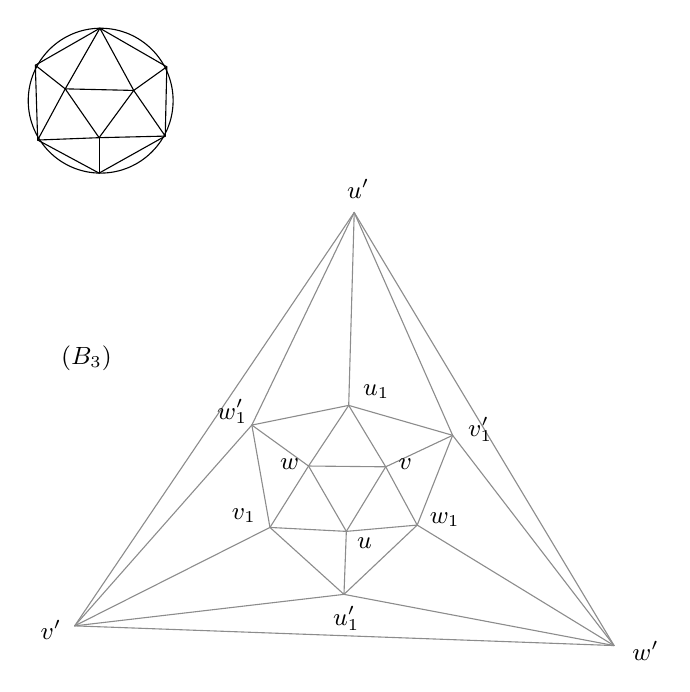
\begin{tikzpicture}[x=1mm,y=1mm,line cap=round,line join=round,font=\scriptsize]
\draw[pencil] (56,-33) -- (43,-60);
\draw[pencil] (56,-33) -- (68.5,-61.3);
\draw[pencil] (20.5,-85.5) -- (43,-60);
\draw[pencil] (20.5,-85.5) -- (54.7,-81.5);
\draw[pencil] (89,-88) -- (68.5,-61.3);
\draw[pencil] (89,-88) -- (54.7,-81.5);
\draw[pencil] (56,-33) -- (55.3,-57.5);
\draw[pencil] (20.5,-85.5) -- (45.3,-73);
\draw[pencil] (89,-88) -- (64,-72.7);
\draw[pencil] (43,-60) -- (55.3,-57.5);
\draw[pencil] (43,-60) -- (45.3,-73);
\draw[pencil] (68.5,-61.3) -- (55.3,-57.5);
\draw[pencil] (68.5,-61.3) -- (64,-72.7);
\draw[pencil] (54.7,-81.5) -- (45.3,-73);
\draw[pencil] (54.7,-81.5) -- (64,-72.7);
\draw[pencil] (50.2,-65.2) -- (55.3,-57.5);
\draw[pencil] (50.2,-65.2) -- (45.3,-73);
\draw[pencil] (60,-65.3) -- (55.3,-57.5);
\draw[pencil] (60,-65.3) -- (64,-72.7);
\draw[pencil] (55,-73.5) -- (45.3,-73);
\draw[pencil] (55,-73.5) -- (64,-72.7);
\draw[pencil] (50.2,-65.2) -- (43,-60);
\draw[pencil] (60,-65.3) -- (68.5,-61.3);
\draw[pencil] (55,-73.5) -- (54.7,-81.5);
\draw[pencil] (50.2,-65.2) -- (60,-65.3);
\draw[pencil] (60,-65.3) -- (55,-73.5);
\draw[pencil] (55,-73.5) -- (50.2,-65.2);
\draw[pencil] (56,-33) -- (20.5,-85.5) -- (89,-88) -- cycle;
\node[inner sep=1pt] at (56.5,-30) {\small $u'$};
\node[inner sep=1pt] at (17.5,-86) {\small $v'$};
\node[inner sep=1pt] at (93,-88.7) {\small $w'$};
\node[inner sep=1pt] at (40.5,-58.3) {\small $w'_1$};
\node[inner sep=1pt] at (58.8,-55.8) {\small $u_1$};
\node[inner sep=1pt] at (72,-60.5) {\small $v'_1$};
\node[inner sep=1pt] at (42,-71.5) {\small $v_1$};
\node[inner sep=1pt] at (67.5,-72) {\small $w_1$};
\node[inner sep=1pt] at (55,-84.5) {\small $u'_1$};
\node[inner sep=1pt] at (47.8,-65) {\small $w$};
\node[inner sep=1pt] at (62.5,-65) {\small $v$};
\node[inner sep=1pt] at (57.3,-75) {\small $u$};
\node[inner sep=1pt] at (22,-51.5) {\small $(B_3)$};
\draw (23.8,-18.8) circle[radius=9.2];
\draw (23.7,-9.6) -- (32.2,-14.5) -- (32,-23.3) -- (23.6,-28) -- (15.8,-23.8) -- (15.5,-14.3) -- cycle;
\draw (19.3,-17.3) -- (28,-17.5) -- (23.6,-23.5) -- cycle;
\draw (19.3,-17.3) -- (15.5,-14.3);
\draw (19.3,-17.3) -- (23.7,-9.6);
\draw (19.3,-17.3) -- (15.8,-23.8);
\draw (28,-17.5) -- (23.7,-9.6);
\draw (28,-17.5) -- (32.2,-14.5);
\draw (28,-17.5) -- (32,-23.3);
\draw (23.6,-23.5) -- (15.8,-23.8);
\draw (23.6,-23.5) -- (23.6,-28);
\draw (23.6,-23.5) -- (32,-23.3);
\end{tikzpicture}
\end{document}
